\documentclass[tikz]{standalone}
%\usepackage[dvipsnames]{xcolor}
\usepackage{amsmath}
\usepackage{amssymb}
\usepackage{setspace}
\usepackage{xeCJK}
\usepackage{ulem}
\usepackage{pstricks}
\usepackage{pstricks-add}
\usepackage{bm}
\usepackage{mathtools}
\usepackage{breqn}
\usepackage{mathrsfs}
\usepackage{esint}
\usepackage{textcomp}
\usepackage{upgreek}
\usepackage{pifont}
\usepackage{tikz}
\usepackage{circuitikz}
\usepackage{caption}
\usepackage{tabularx}
\usepackage{array}
\usepackage{pgfplots}
\usepackage{multirow}
\usepackage{pgfplotstable}
\usepackage{mhchem}

\setCJKfamilyfont{boldsong}[AutoFakeBold = {2.17}]{SimSun}
\newcommand*{\boldsong}{\CJKfamily{boldsong}}
%\DeclareMathOperator\dif{d\!}
\newcommand*{\me}{\mathop{}\!\mathrm{e}}
\newcommand*{\mpar}{\mathop{}\!\partial}
\newcommand*{\dif}{\mathop{}\!\mathrm{d}}
\newcommand*{\tab}{\indent}
\newcommand*{\mcelsius}{\mathop{}\!{^\circ}\mathrm{C}}
\renewcommand*{\Im}{\mathrm{Im}\,}

\begin{document}
	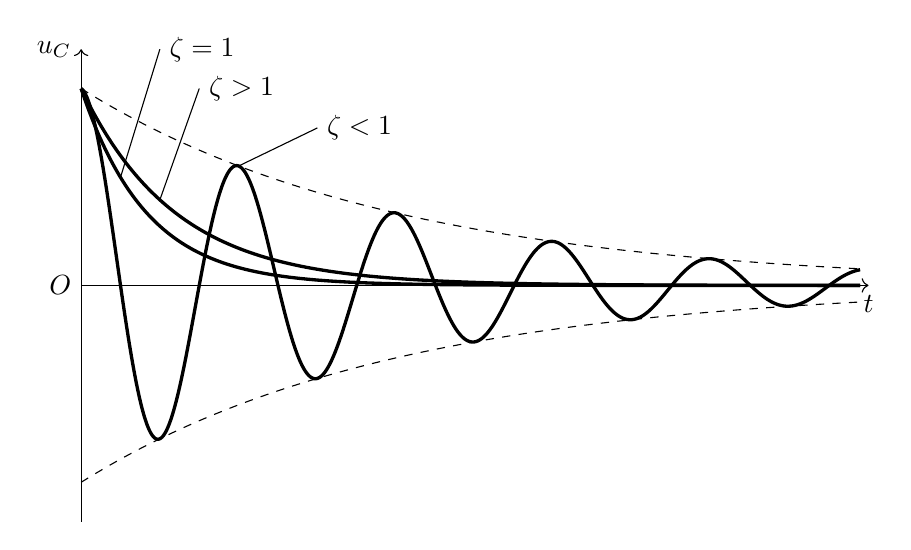
\begin{tikzpicture}
		\draw[->] (0,-3)--(0,3)node[left]{$ u_C $};
		\draw[->] (0,0)node[left]{$ O $}--(10,0)node[below]{$ t $};
		\draw[very thick,domain=0:9.9,samples=1000] plot (\x,{2.5*exp(-\x/4)*cos(pi*\x r)});
		\draw[dashed,domain=0:9.9,samples=1000] plot (\x,{2.5*exp(-\x/4)});
		\draw[dashed,domain=0:9.9,samples=1000] plot (\x,{-2.5*exp(-\x/4)});
		\draw[very thick,domain=0:9.9,samples=1000] plot (\x,{2.5*exp(-\x*1.2)});
		\draw[very thick,domain=0:9.9,samples=1000] plot (\x,{2.5*exp(-\x/1.2)});
		\draw (0.5,1.372)--(1,3)node[right]{$ \zeta=1 $};
		\draw (1,1.0865)--(1.5,2.5)node[right]{$ \zeta>1 $};
		\draw (2,1.5163)--(3,2)node[right]{$ \zeta<1 $};
	\end{tikzpicture}
\end{document}